%!TEX root = ../main.tex
\subsubsection{Banach spaces}

\begin{defn}
	A normed vector space $(X,\norm{\cdot})$ is a \emph{Banach space} if it is complete\footnotemark{} with respect to the metric induced by the norm.
\end{defn}
\footnotetext{See definition \vref{complete-space-defn}, a metric space is complete if any fundamental sequence converges.}

Here a first but relevant observation.
\begin{prop}
	Every closed subspace of a Banach space is a Banach space itself.
\end{prop}

Consider now some examples.
\begin{exam}
	The normed vector spaces $(\RR^N, \norm{\cdot}_p)$ are Banach spaces $\forall p \in [1,\infty]$. All those norms are equivalent each other.
\end{exam}
\begin{exam}
	The normed vector spaces $(l^p,\norm{\cdot}_p)$ are Banach spaces $\forall p \in [1,\infty]$.
\end{exam}
\begin{exam}
	The normed vector space of the continuous functions $(\Cc([a,b]),\norm{\cdot}_\infty)$ is a Banach space. Indeed, if $\norm{f_n-f}\to 0$, then:
	$$
	\forall \eps 
	> 0 
	\ \exists
	\, n_0
	=n_0(\eps) 
	\in \NN 
	: \quad	|f_n(t)-f(t)|
	\leq \max_{t \in [a,b]} |f_n(t)-f(t)| 
	< \eps
	.
	$$
	Moreover, as $\norm{\cdot}_\infty$ is not equivalent to the integral norm $\norm{\cdot}_1$, $(X, \norm{\cdot}_1)$ is not a Banach space.\\
	In $X=\Cc^1([a,b])$ the norm $\norm{\cdot}_{\infty, 1}$ is equivalent to:
	$$
	\norm{f} 
	= |f(a)| + \norm{f'}_\infty
	.
	$$
\end{exam}
\begin{exam}
	Let $k\in \NN_0$ and define the following space:
	$$
	\Cc^k([a,b]) 
	\coloneqq \{
		f:[a,b]\to \RR : 
		f^{(i)}\in \Cc([a,b]) \ 
		\forall i = 1,\ldots,k 
	\}
	.
	$$
	Its norm is
	$$
	\norm{f}_{\infty,k}
	\coloneqq 
	\sum_{j=0}^{k} \norm{f^{(i)}}_\infty
	.
	$$
	Then $(\Cc^k([a,b]),\norm{\cdot}_{\infty,k})$ are Banach spaces.
\end{exam}
\begin{exam}
	Consider the following space:
	$$\Cc^\infty([a,b]) \coloneqq \{f:[a,b]\to \RR : \exists\; f^{(i)} \in \Cc ([a,b]) \ \forall i\in \NN \}.$$
	It is a vector space, but there does not exist a norm such that it becomes a Banach space. However, it is a complete metric space with the norm:
	$$d_\infty(f,g) = \sum_{j=0}^\infty 2^{-j} \frac{\norm{f^{(j)}-g^{(j)}}_\infty}{1+\norm{f^{(j)}-g^{(j)}}_\infty}.$$
\end{exam}

Also the space of absolute continuous function is Banach.
\begin{exam}
	Let $X = AC[a,b]$. You should prove that 
	$$
	\norm{f}_\star 
	= |f(a)| + \norm{f'}_1
	$$ 
	is a norm in $X$, then see the next.
	
	Here we prove that $(AC([a,b]), \norm{\cdot}_\star)$ is a Banach space.\\
	Consider a fundamental sequence of absolute continuous function $\{f_n\}_{n\in \NN}$. We have to check that this sequence converges to an absolute continuous function.\\
	Take the sequence $\{f_n(a)\}_{n\in\NN}$, it is fundamental and converges in $(\RR, \abs{\cdot})$, so we write $f_n(a) \to \alpha$.\\
	Consider also $\{f_n'\}_{n\in\NN}$, it's fundamental as well and exists $g \in L^1([a,b])$ such that $\norm{f_n - g}_1 \to 0$ for $n \to \infty$.
	
	By calculus formula we have a relation between those sequences, indeed:
	$$
	f_n(t) 
	= f_n(a) + \int_a^t f_n'(\tau) \de \tau 
	\quad t 
	\in [a,b]
	.
	$$
	As $f_n'$ converges to $g$, it does also the integral, indeed, for all $t \in [a,b]$ we have:
	$$
	\left| \; \int_a^t(f_n'-g)(\tau) \de \tau \; \right|
	\leq \int_a^b \left | \; (f_n'-g)(\tau) \right| \de \tau
	=  \norm{f_n' -g}_1 \to 0
	\quad \text{as}
	\quad n
	\to \infty
	.
	$$
	This implies that $f_n$ converges point-wise (and uniformly) in $[a,b]$ to a function $f$ defined by:
	$$
	f(t) 
	= \alpha + \int_a^t g(\tau)\de\tau
	\quad t 
	\in [a,b]
	,
	$$
	so that $f(a)= \alpha$ and $f' = g$ a.e. in $[a,b]$.\\
	By properties of absolutely continuous functions (see, in particular, \vref{theo-abs-continuity-int}), $f \in AC([a,b])$ and $\norm{f_n - f}_\star \to 0$ as $n \to \infty$.\\
	Hence, $(AC([a,b]), \norm{\cdot}_\star)$ is a Banach space.
	
	Moreover, $AC([a,b])$ the following norm is equivalent to the one we present:
	$$
	\norm{f} 
	= |f(a)| + \norm{f'}_1
	;
	$$
	also this norm makes $AC([a,b])$ a Banach space.
\end{exam}

\begin{exam}
		The space $BV([a,b])$ is a Banach space with respect to the norm 
		$$
		\norm{f} 
		= \norm{f}_1 + \tv^b_a (f)
		,
		$$
		but $\norm{\cdot}_{AC}$ is not a norm in $X$.
\end{exam}


Finally, notice that in an infinite dimensional vector space it's possible to construct non-equivalent norms such that all of them make it a Banach space.

\paragraph{Schauder bases} Similarly to the algebraic basis for vector space, can we write any element of a Banach space as a sum of a series of a given sequence of elements? Yes, what we obtain is a sort of weak version of the algebraic basis, as we will see this new basis is for a set which is dense in the original space.

\begin{defn}
	Let $(X,\norm{\cdot})$ be a normed vector space on $\RR$, $\{x_n\}_{n \in \NN}\subset X$, and set:
	$$E = \left\{\sum_{n=0}^k \alpha_n x_n : \ \alpha_0, \ldots, \alpha_k \in \RR, \  k\in \NN \right\}.$$
	Then the sequence $\{x_n\}_{n \in \NN}$ is a \emph{Schauder basis} if $E$ is dense in $X$.
\end{defn}

In other words, a sequence is a Schauder basis in $X$ if the set of its finite linear combinations with rational coefficients is dense in $X$.

One can easily figure out the following result:
\begin{prop}
	If a normed vector space has a Schauder basis, then it is separable.
\end{prop}  
In general, the reverse is not true.\footnote{Proved by Per Henrik Enflo (Stockholm, 1944) in 1975. Thanks to this proof, he won a goose as a prize.}

Observe that $\{x^n\}_{n \in \NN}$ is a Schauder basis for $(\Cc([a,b]),\norm{\cdot}_\infty)$ (see the Stone--Weierstrass theorem \vref{theo-stone-weierstrass}).


\paragraph{Characterization of Banach spaces} Here we provide one characterization through the following theorem. It states that a normed vector space $(X,\norm{\cdot})$ is a Banach space if and only if any absolutely convergent series converges in $X$.\footnote{Remember that a series $\sum_{n\in\NN} x_n$ converges absolutely if $\sum_{n\in\NN}\norm{x_n}$ converges.}

\begin{theo} \label{theo-banach-space-charact}
	Let $(X, \norm{\cdot})$ be a normed vector space. \\
	Then:
	$$
		{\scriptstyle (X,\norm{\cdot})\ \text{is a B-space} \iff \left[\forall \{x_n\}_{n\in\NN} \subset X,\ \ \sum_{n\in\NN} \norm{x_n} < +\infty \implies \sum_{n \in \NN} x_n < +\infty \right]}
	$$
\end{theo}

\begin{proof}\textit{Necessary condition} $\implies$:\\
	Having that $(X, \norm{\cdot})$ is Banach, it's enough to prove that $\sum_{n\in\NN} x_n$ is fundamental. Again by hypothesis, $\sum_{n\in\NN} \norm{x_n} < +\infty$.\\
	Define $S_n = \sum_{i=0}^{n} x_i$; taking $m > n$, we have:
	$$\norm{ S_m - S_n}
	= \norm{\sum_{i=n+1}^m x_i} 
	\leq \sum^m_{i=n+1}\norm{x_i}
	\to 0
	\quad \text{as}
	\quad n,m \to +\infty 
	;
	$$
	hence $\sum_{n\in\NN} x_n$ is fundamental and, being in a Banach space, it converges.
		
	\textit{Sufficient condition} $\impliedby$:\\
	Consider a Cauchy sequence $\{x_n\}_{n \in \NN}$.
	We can construct a sub-sequence $\{x_{n_h}\}_{h \in \NN_0}$ such that:
	$$
	\norm{x_{n_{h+1}}-x_{n_h}}
	\leq \frac 1{h^2} 
	\quad \forall h \in \NN_0
	.
	$$
	Then, by hypothesis, the series $\sum_{h\in\NN_0} (x_{n_{h+1}}-x_{n_h})$, which is telescopic, converges to some $x \in X$, and so the sequence of partial sums does:
	$$
	S_{h+1} = 
	x_{n_{h+1}}-x_{n_1} 
	\to x 
	\in X 
	\quad \text{as } 
	h
	\to \infty
	,
	$$
	which means $x_{n_{h+1}} \to x+x_{n_1} \in X$ as $h\to \infty$.\\
	From a known result, since we had a Cauchy sequence and we've been able to extract a converging subsequence, then also the Cauchy sequence converges, namely $\{x_n\}_{n \in \NN}$ converges.
\end{proof}

\paragraph{Finite dimensional Banach spaces} Here we have another topological notion that we will try to analyze in the context of Banach spaces. We have seen this property yet, recall definitions of compact space \vref{compact-space-defn} and sequentially compact space \vref{seq-compact-space-defn}, as well Bolzano--Weierstrass theorem \vref{bolzano-weierstrass-theo}, the theorem of characterization of compact spaces \vref{characterization-compact-spaces} and Heine--Borel's \vref{heine-borel-theo}. 

Bolzano--Weierstrass states that in a metric space on $\RR^N$, with any metric, from any bounded sequence can be extracted a converging subsequence. Now we know that some metrics coupled with $\RR^N$ constitutes a Banach space. The following theorem uses the ``Bolzano--Weierstrass'' property to characterize finite-dimensional Banach spaces.

\begin{theo}[characterization of finite-dimensional Banach spaces] \label{characterization-finite-banach-theo}
	A Banach space $(X,\norm{\cdot})$ is finite-dimensional if and only if from any bounded sequence it is possible to extract a converging subsequence.
\end{theo}

\paragraph{Frederic Riesz's theorem}\footnotemark{} From the previous results we can deduce that any compact set in a Banach space is closed and bounded. The following result try to understand how the  converse can be true, and an answer is provided by its corollaries.
\footnotetext{Frigyes Riesz was an hungarian mathematician whose name is often spelled ``Frederic''. Other Riesz theorem are named after his younger brother Marcel.}

\begin{theo}[Frederic Riesz]\label{theorem-riesz}
	Let $(X, \norm{\cdot})$ be a a normed vector space.\\
	If the closure of the unit ball $B \subset X$ is compact then $X$ is finite-dimensional.
\end{theo}

To prove this we will use the following.

\begin{lemm}
	If $(X, \norm{\cdot})$ is a normed vector space and $Y \subsetneq X$ is a closed (linear) subspace then, for all $\varepsilon > 0$, there exists $x \in X$ such that:
	$$
	\norm{x} 
	= 1 
	\quad \text{and} 
	\quad d(x,y) 
	\geq 1 - \varepsilon
	\quad \forall y \in Y
	.
	$$
\end{lemm} 

\begin{proof}
	Let $y \in X \setminus Y$, and fix $y \in Y$. We have that $d(y,Y) = \norm{x -y} > 0$ as $Y$ is closed.\\
	Suppose that $\varepsilon \in (0,1)$, then choose $z \in Y$ for which:
	$$ 
	d
	\leq \norm{y-z} 
	\leq \frac{d}{1-\varepsilon}
	.
	$$
	Setting:
	$$
	x 
	= \frac{y-z}{\norm{y-z}}
	\notin Y,
	$$
	we have for any $u \in Y$ that:
	$$ 
	\norm{x-u} 
	= \norm{ \frac{y-z}{\norm{y-z}} - u } 
	\geq \frac{d}{\norm{y-z}} 
	\geq 1-\varepsilon
	,
	$$
	since $z + \norm{y-z}u \in Y$.
	
	If $\varepsilon > 1$ then the proof is trivial.
\end{proof} 

Now we can proceed.

\begin{proof}[Proof of the Frederic Riesz's theorem.]
	By contradiction suppose that $X$ is infinite-dimensional.\\
	Then we can find a sequence of finite-dimensional subspaces $\{E_n\}_{n\in \NN}$ such that $E_{n-1} \subsetneq E_n.$\\
	Thanks to the previous lemma, we can construct a sequence $\{x_n\}_{n \in \NN}$ picking up an element from each set as follows:
	$$x_n \in E_n, \quad \norm{x_n} = 1, \quad d(x_n, E_{n-1})\geq \frac{1}{2}.$$
	In particular, we have $\norm{x_n - x_m} \geq \frac 1 2$ for $n \neq m$. This means that $\{x_n\}_{n \in \NN}$ is bounded but has no convergent sequence. This is a contradiction with the characterization of finite-dimensional Banach spaces (see theorem \vref{characterization-finite-banach-theo}), so the proof is complete.
\end{proof}

Frederic Riesz's theorem has many consequences.

\begin{coro}
	A Banach space if finite-dimensional if and only if any bounded and closed subset is compact. 
\end{coro}

\begin{coro}
	Let $(X, \norm{\cdot})$ be an infinite-dimensional normed vector space.\\ 
	Then any compact set has an empty interior; that is it doesn't contains any ball.
\end{coro}

\paragraph{A compactness criterion for the space of continuous functions} Our goal now is to deduce a compactness criterion for the \textit{infinite-dimensional} Banach spaces of continuous functions. The following theorem is the first step.

\begin{theo}[Ascoli--Arzelà] \label{theo-ascoli-arzela}
	Consider the metric space $(\Cc([a,b]),\norm{\cdot}_\infty)$, and let $\{f_n\}_{n \in \NN} \subset \Cc([a,b])$.\\
	If $\{f_n\}_{n \in \NN}$ is:
	\begin{itemize}
		\item\emph{bounded}, namely:
		$$
		\exists \, M > 0 : \quad 
		\sup_{n \in \NN} \norm{f_n}_\infty 
		\leq M
		;
		$$
		\item\emph{equicontinuous}, namely:
		\begin{align*}
		&\forall \eps > 0 \ 
		\exists \, \delta = \delta (\eps) > 0:\\
		&\forall t_1, t_2 \in [a,b] : 
		\ |t_1-t_2|< \delta
		\implies
		|f_n(t_1)-f_n(t_2)|
		<\eps
		\quad \forall n 
		\in \NN
		;
		\end{align*}
	\end{itemize}
	then there exists a subsequence $\{f_{n_h}\}_{h\in\NN}$ such that $f_{n_h} \to f$ in $(\Cc([a,b]), \norm{\cdot}_\infty)$.
\end{theo}

Notice that as $f_{n_h} \to f$ in norm $\norm{\cdot}_\infty$, the convergence is uniform.


\begin{proof}
	The goal of this proof is to extract a subsequence which converges uniformly, that is a convergence with respect to the infinity norm.
	
	\textit{Step 1}: Let $\{q_j\}_{j\in\NN}$ be an enumeration of $\QQ \cap [a,b]$.
	
	Consider first $\{f_n(q_0)\}_{n \in \NN}$: because of boundedness, it is bounded in $\RR$, so we can use Bolzano--Weierstrass (see theorem \vref{bolzano-weierstrass-theo}) and assert that there exists a subsequence $\{f_{n_{k_0}}(q_0)\}_{k_0\in\NN}$ which converges.
	
	Consider now $\{f_{n_{k_0}}(q_1)\}_{k_0 \in \NN}$: it is bounded as well, and there exists $\{f_{n_{k_1}} (q_1)\}_{k_1 \in \NN}$ which converges.

	Notice that $\{f_{n_{k_1}}(q_0)\}_{k_1 \in \NN}$ also converges.
	
	Repeating this argument for every element in $\{q_j\}_{j \in \NN}$ using a Cantor diagonalization argument (the one used to prove that $\QQ$ is countable), we get a sequence of functions $\{f_{n_h}(t)\}_{h \in \NN}$ which converges point-wise for $t = q_j$.

	\begin{figure}[htpb]
		\centering
		\tikzset{every picture/.style={line width=0.75pt}} %set default line width to 0.75pt        

		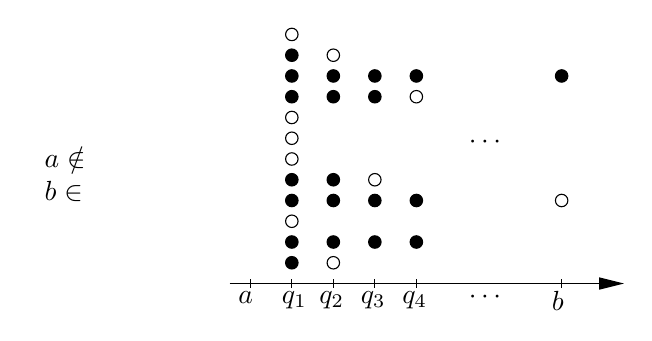
\begin{tikzpicture}[x=0.75pt,y=0.75pt,yscale=-1,xscale=1]
		%uncomment if require: \path (0,300); %set diagram left start at 0, and has height of 300

		\draw    (130,180) -- (318,180) ;
		\draw [shift={(320,180)}, rotate = 180] [fill={rgb, 255:red, 0; green, 0; blue, 0 }  ][line width=0.08]  [draw opacity=0] (12,-3) -- (0,0) -- (12,3) -- cycle    ;
		\draw  [fill={rgb, 255:red, 0; green, 0; blue, 0 }  ,fill opacity=1 ] (157,170) .. controls (157,168.34) and (158.34,167) .. (160,167) .. controls (161.66,167) and (163,168.34) .. (163,170) .. controls (163,171.66) and (161.66,173) .. (160,173) .. controls (158.34,173) and (157,171.66) .. (157,170) -- cycle ;
		\draw  [fill={rgb, 255:red, 0; green, 0; blue, 0 }  ,fill opacity=1 ] (157,160) .. controls (157,158.34) and (158.34,157) .. (160,157) .. controls (161.66,157) and (163,158.34) .. (163,160) .. controls (163,161.66) and (161.66,163) .. (160,163) .. controls (158.34,163) and (157,161.66) .. (157,160) -- cycle ;
		\draw   (157,150) .. controls (157,148.34) and (158.34,147) .. (160,147) .. controls (161.66,147) and (163,148.34) .. (163,150) .. controls (163,151.66) and (161.66,153) .. (160,153) .. controls (158.34,153) and (157,151.66) .. (157,150) -- cycle ;
		\draw  [fill={rgb, 255:red, 0; green, 0; blue, 0 }  ,fill opacity=1 ] (157,140) .. controls (157,138.34) and (158.34,137) .. (160,137) .. controls (161.66,137) and (163,138.34) .. (163,140) .. controls (163,141.66) and (161.66,143) .. (160,143) .. controls (158.34,143) and (157,141.66) .. (157,140) -- cycle ;
		\draw  [fill={rgb, 255:red, 0; green, 0; blue, 0 }  ,fill opacity=1 ] (157,130) .. controls (157,128.34) and (158.34,127) .. (160,127) .. controls (161.66,127) and (163,128.34) .. (163,130) .. controls (163,131.66) and (161.66,133) .. (160,133) .. controls (158.34,133) and (157,131.66) .. (157,130) -- cycle ;
		\draw   (157,120) .. controls (157,118.34) and (158.34,117) .. (160,117) .. controls (161.66,117) and (163,118.34) .. (163,120) .. controls (163,121.66) and (161.66,123) .. (160,123) .. controls (158.34,123) and (157,121.66) .. (157,120) -- cycle ;
		\draw   (157,110) .. controls (157,108.34) and (158.34,107) .. (160,107) .. controls (161.66,107) and (163,108.34) .. (163,110) .. controls (163,111.66) and (161.66,113) .. (160,113) .. controls (158.34,113) and (157,111.66) .. (157,110) -- cycle ;
		\draw   (157,100) .. controls (157,98.34) and (158.34,97) .. (160,97) .. controls (161.66,97) and (163,98.34) .. (163,100) .. controls (163,101.66) and (161.66,103) .. (160,103) .. controls (158.34,103) and (157,101.66) .. (157,100) -- cycle ;
		\draw  [fill={rgb, 255:red, 0; green, 0; blue, 0 }  ,fill opacity=1 ] (157,90) .. controls (157,88.34) and (158.34,87) .. (160,87) .. controls (161.66,87) and (163,88.34) .. (163,90) .. controls (163,91.66) and (161.66,93) .. (160,93) .. controls (158.34,93) and (157,91.66) .. (157,90) -- cycle ;
		\draw  [fill={rgb, 255:red, 0; green, 0; blue, 0 }  ,fill opacity=1 ] (157,80) .. controls (157,78.34) and (158.34,77) .. (160,77) .. controls (161.66,77) and (163,78.34) .. (163,80) .. controls (163,81.66) and (161.66,83) .. (160,83) .. controls (158.34,83) and (157,81.66) .. (157,80) -- cycle ;
		\draw  [fill={rgb, 255:red, 0; green, 0; blue, 0 }  ,fill opacity=1 ] (157,70) .. controls (157,68.34) and (158.34,67) .. (160,67) .. controls (161.66,67) and (163,68.34) .. (163,70) .. controls (163,71.66) and (161.66,73) .. (160,73) .. controls (158.34,73) and (157,71.66) .. (157,70) -- cycle ;
		\draw   (157,60) .. controls (157,58.34) and (158.34,57) .. (160,57) .. controls (161.66,57) and (163,58.34) .. (163,60) .. controls (163,61.66) and (161.66,63) .. (160,63) .. controls (158.34,63) and (157,61.66) .. (157,60) -- cycle ;
		\draw   (177,170) .. controls (177,168.34) and (178.34,167) .. (180,167) .. controls (181.66,167) and (183,168.34) .. (183,170) .. controls (183,171.66) and (181.66,173) .. (180,173) .. controls (178.34,173) and (177,171.66) .. (177,170) -- cycle ;
		\draw  [fill={rgb, 255:red, 0; green, 0; blue, 0 }  ,fill opacity=1 ] (177,160) .. controls (177,158.34) and (178.34,157) .. (180,157) .. controls (181.66,157) and (183,158.34) .. (183,160) .. controls (183,161.66) and (181.66,163) .. (180,163) .. controls (178.34,163) and (177,161.66) .. (177,160) -- cycle ;
		\draw  [fill={rgb, 255:red, 0; green, 0; blue, 0 }  ,fill opacity=1 ] (177,140) .. controls (177,138.34) and (178.34,137) .. (180,137) .. controls (181.66,137) and (183,138.34) .. (183,140) .. controls (183,141.66) and (181.66,143) .. (180,143) .. controls (178.34,143) and (177,141.66) .. (177,140) -- cycle ;
		\draw  [fill={rgb, 255:red, 0; green, 0; blue, 0 }  ,fill opacity=1 ] (177,130) .. controls (177,128.34) and (178.34,127) .. (180,127) .. controls (181.66,127) and (183,128.34) .. (183,130) .. controls (183,131.66) and (181.66,133) .. (180,133) .. controls (178.34,133) and (177,131.66) .. (177,130) -- cycle ;
		\draw  [fill={rgb, 255:red, 0; green, 0; blue, 0 }  ,fill opacity=1 ] (177,90) .. controls (177,88.34) and (178.34,87) .. (180,87) .. controls (181.66,87) and (183,88.34) .. (183,90) .. controls (183,91.66) and (181.66,93) .. (180,93) .. controls (178.34,93) and (177,91.66) .. (177,90) -- cycle ;
		\draw  [fill={rgb, 255:red, 0; green, 0; blue, 0 }  ,fill opacity=1 ] (177,80) .. controls (177,78.34) and (178.34,77) .. (180,77) .. controls (181.66,77) and (183,78.34) .. (183,80) .. controls (183,81.66) and (181.66,83) .. (180,83) .. controls (178.34,83) and (177,81.66) .. (177,80) -- cycle ;
		\draw   (177,70) .. controls (177,68.34) and (178.34,67) .. (180,67) .. controls (181.66,67) and (183,68.34) .. (183,70) .. controls (183,71.66) and (181.66,73) .. (180,73) .. controls (178.34,73) and (177,71.66) .. (177,70) -- cycle ;
		\draw  [fill={rgb, 255:red, 0; green, 0; blue, 0 }  ,fill opacity=1 ] (197,160) .. controls (197,158.34) and (198.34,157) .. (200,157) .. controls (201.66,157) and (203,158.34) .. (203,160) .. controls (203,161.66) and (201.66,163) .. (200,163) .. controls (198.34,163) and (197,161.66) .. (197,160) -- cycle ;
		\draw  [fill={rgb, 255:red, 0; green, 0; blue, 0 }  ,fill opacity=1 ] (197,140) .. controls (197,138.34) and (198.34,137) .. (200,137) .. controls (201.66,137) and (203,138.34) .. (203,140) .. controls (203,141.66) and (201.66,143) .. (200,143) .. controls (198.34,143) and (197,141.66) .. (197,140) -- cycle ;
		\draw   (197,130) .. controls (197,128.34) and (198.34,127) .. (200,127) .. controls (201.66,127) and (203,128.34) .. (203,130) .. controls (203,131.66) and (201.66,133) .. (200,133) .. controls (198.34,133) and (197,131.66) .. (197,130) -- cycle ;
		\draw  [fill={rgb, 255:red, 0; green, 0; blue, 0 }  ,fill opacity=1 ] (197,80) .. controls (197,78.34) and (198.34,77) .. (200,77) .. controls (201.66,77) and (203,78.34) .. (203,80) .. controls (203,81.66) and (201.66,83) .. (200,83) .. controls (198.34,83) and (197,81.66) .. (197,80) -- cycle ;
		\draw  [fill={rgb, 255:red, 0; green, 0; blue, 0 }  ,fill opacity=1 ] (217,160) .. controls (217,158.34) and (218.34,157) .. (220,157) .. controls (221.66,157) and (223,158.34) .. (223,160) .. controls (223,161.66) and (221.66,163) .. (220,163) .. controls (218.34,163) and (217,161.66) .. (217,160) -- cycle ;
		\draw   (217,90) .. controls (217,88.34) and (218.34,87) .. (220,87) .. controls (221.66,87) and (223,88.34) .. (223,90) .. controls (223,91.66) and (221.66,93) .. (220,93) .. controls (218.34,93) and (217,91.66) .. (217,90) -- cycle ;
		\draw  [fill={rgb, 255:red, 0; green, 0; blue, 0 }  ,fill opacity=1 ] (217,80) .. controls (217,78.34) and (218.34,77) .. (220,77) .. controls (221.66,77) and (223,78.34) .. (223,80) .. controls (223,81.66) and (221.66,83) .. (220,83) .. controls (218.34,83) and (217,81.66) .. (217,80) -- cycle ;
		\draw    (160,178) -- (160,182) ;
		\draw    (180,178) -- (180,182) ;
		\draw    (200,178) -- (200,182) ;
		\draw    (220,178) -- (220,182) ;
		\draw    (140,178) -- (140,182) ;
		\draw    (290,178) -- (290,182) ;
		\draw   (287,140) .. controls (287,138.34) and (288.34,137) .. (290,137) .. controls (291.66,137) and (293,138.34) .. (293,140) .. controls (293,141.66) and (291.66,143) .. (290,143) .. controls (288.34,143) and (287,141.66) .. (287,140) -- cycle ;
		\draw  [fill={rgb, 255:red, 0; green, 0; blue, 0 }  ,fill opacity=1 ] (287,80) .. controls (287,78.34) and (288.34,77) .. (290,77) .. controls (291.66,77) and (293,78.34) .. (293,80) .. controls (293,81.66) and (291.66,83) .. (290,83) .. controls (288.34,83) and (287,81.66) .. (287,80) -- cycle ;
		\draw  [fill={rgb, 255:red, 0; green, 0; blue, 0 }  ,fill opacity=1 ] (197,90) .. controls (197,88.34) and (198.34,87) .. (200,87) .. controls (201.66,87) and (203,88.34) .. (203,90) .. controls (203,91.66) and (201.66,93) .. (200,93) .. controls (198.34,93) and (197,91.66) .. (197,90) -- cycle ;
		\draw  [fill={rgb, 255:red, 0; green, 0; blue, 0 }  ,fill opacity=1 ] (217,140) .. controls (217,138.34) and (218.34,137) .. (220,137) .. controls (221.66,137) and (223,138.34) .. (223,140) .. controls (223,141.66) and (221.66,143) .. (220,143) .. controls (218.34,143) and (217,141.66) .. (217,140) -- cycle ;

		\draw (154,182.4) node [anchor=north west][inner sep=0.75pt]    {$q_{1}$};
		\draw (284,182.4) node [anchor=north west][inner sep=0.75pt]    {$b$};
		\draw (172,182.4) node [anchor=north west][inner sep=0.75pt]    {$q_{2}$};
		\draw (192,182.4) node [anchor=north west][inner sep=0.75pt]    {$q_{3}$};
		\draw (212,182.4) node [anchor=north west][inner sep=0.75pt]    {$q_{4}$};
		\draw (244,182.4) node [anchor=north west][inner sep=0.75pt]    {$\cdots $};
		\draw (133,182.4) node [anchor=north west][inner sep=0.75pt]    {$a$};
		\draw (244,107.9) node [anchor=north west][inner sep=0.75pt]    {$\cdots $};
		\draw (33,111.4) node [anchor=north west][inner sep=0.75pt]    {$ \begin{array}{l}
		a\notin \QQ\\
		b\in \QQ
		\end{array}$};
		\end{tikzpicture}
	\end{figure}
	\FloatBarrier
	
	\textit{Step 2}: Then fix $\eps > 0$. Via equicontinuity, we find $\delta=\delta(\eps)>0$ such that: $$|f_{n_h}(t_1)-f_{n_h}(t_2)|<\tfrac{\eps}{3} \quad \forall t_1,t_2 \in [a,b] :|t_1-t_2|<\delta \quad \forall h \in \NN.$$
	
	Consider now a family of intervals $I_i=\{[a_j, b_j]\}^N_{j=1}$ such that $b_j-a_j < \delta$ and $\cup_{j=1}^N [a_j,b_j]=[a,b]$. Then, for any $i$, we can choose $q_i \in I_i$, because $\QQ$ is dense in $\RR$.
	
	Observe that there exists $h_0(\eps) \in \NN$, independent of $j$, such that\footnote{Since this can be done for any $j$, it's enough to take the biggest, as $N$ is finite.}:
	$$|f_{n_h}(q_j)-f_{n_{h'}}(q_j)|\leq \tfrac{\eps}{3} \quad \forall h,h' > h_0 \quad \forall j = 1, \ldots, N.$$
	
	\textit{Step 3}: Let $t\in[a,b]$. Then $t \in I_i$ for some $i \in 1:N$, thus $|t-q_i|<\delta$. Therefore we have, for any $h, h'>h_0$:
	\begin{align*}
	|f_{n_h}(t)-f_{n_{h'}}(t)|
	&\leq |f_{n_h}(t)-f_{n_h}(q_j)|+|f_{n_h}(q_j)-f_{n_{h'}}(q_j)|+|f_{n_{h'}}(q_j)-f_{n_{h'}}(t)| \\
	&\le \tfrac{\eps}{3}+\tfrac{\eps}{3}+\tfrac{\eps}{3}\\
	&= \eps
	\end{align*}
	
	Thus $\{f_{n_h}\}$ is a uniform Cauchy sequence, that is a Cauchy sequence with respect to $\norm{\cdot}_\infty$, and it converges in the Banach space $(\Cc([a,b]),\norm{\cdot}_\infty)$.
\end{proof}


Also it can be shown that the boundedness and equicontinuity are also necessary for compactness in $(\Cc([a,b]), \norm{\cdot}_\infty)$.

Actually, equicontinuity and equiboundedness are also necessary conditions: namely, if $K \subset \Cc([a,b])$ is compact, then any $\{f_n\}\subset K$ satisfies them.

How this theorem is related to compactness? Apparently in the theorem formulation there is no mention to compactness but we see in the following example that exists a strong relation.

\begin{exam}
	Consider the following subset of $(\Cc([a,b]), \norm{\cdot}_\infty)$: 
	$$ 
	E_M 
	= \{
	f \in \Cc^1([a,b]) :\ 
	\norm{f}_\infty + \norm{f'}_\infty \leq M
	\}
	$$
	for some given $M > 0$.
	
	Thanks to the Ascoli--Arzelà theorem, we can prove that $E_M$ is sequentially compact, and so it is also compact. Indeed, take a sequence $\{f_n\}_{n\in \NN} \subset E_M$: it is bounded and, owing to the Lagrange theorem, we have: 
	$$
	\abs{f_n(x) - f_n(y)} 
	\leq M \abs{x-y} 
	\quad \forall x,y \in [a,b], \ 
	\forall n \in \NN
	.
	$$
	Thus the sequence is also equicontinuous so it contains a subsequence which converges uniformly to some $f \in E_M$.
\end{exam}





